\documentclass[11pt]{article}
\usepackage{enumitem}
\usepackage{amsmath,amsthm,amssymb}
\usepackage{color}
\usepackage{graphicx}
\graphicspath{ {./images/} }

\begin{document}
\date{} 
\title{Lab Report 4\\--\\\large CPE282 Fall 2020}
\author{Brennen Green}
\maketitle

\section*{Rock Paper Scissors}
This section was somewhat difficult at first. I really had to rewatch the videos and look at
the code a few times to understand what was going on. Once I understand what the verilog design
and constraints were doing, and how I could manipulate them it became a lot more straightfoward
and from there I just continued to follow the video pretty closely to finish up.
\begin{center}
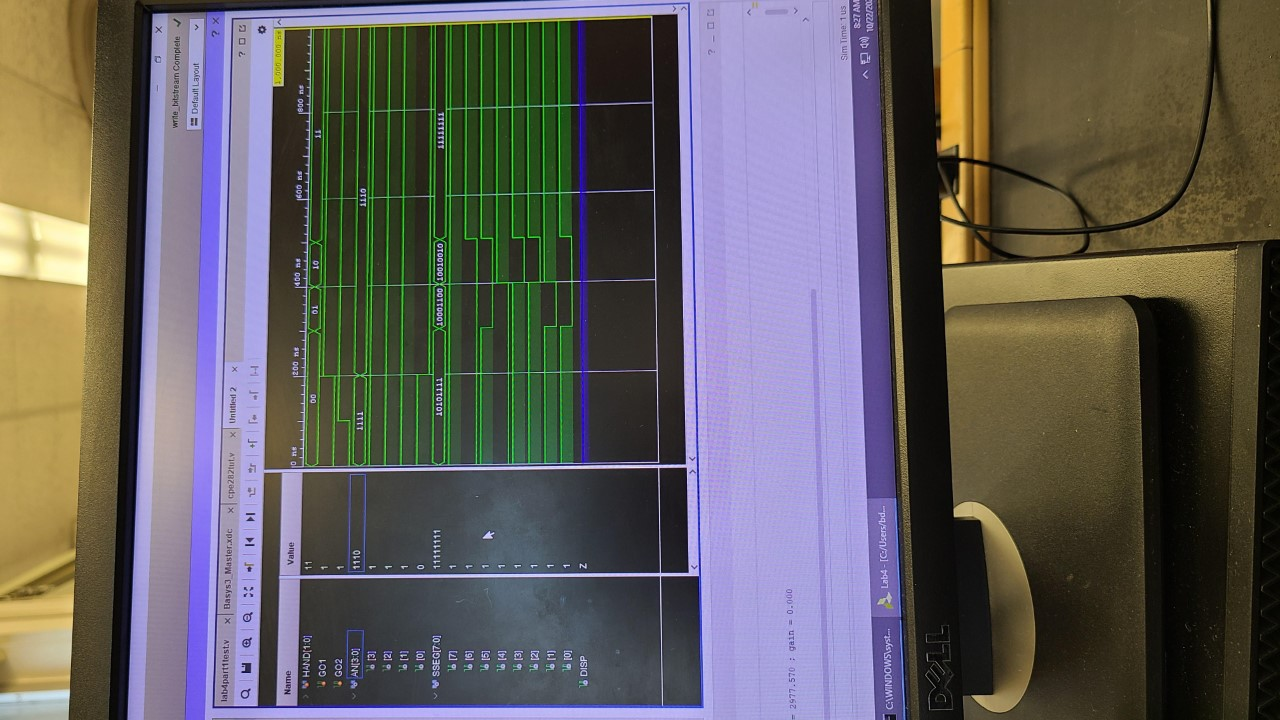
\includegraphics[width=15cm,height=15cm]{rps_sim}\newline
(Rock Paper Scissors Simulation)
\end{center}
\section*{7 Segment Number}
This section was a lot smoother because of what I learned from the previous section. Without
having to rewrite a ton of code, I just reused the code already written in the previous section
and manipulated multiple variables such as the HAND input and the final SSEG output of the program.
\begin{verbatim}
    `timescale 1ns / 1ps

//A simple verilog module representing the player input of a rock,paper,scissors game.
// Used as an example for learning Vivado in CPE/EE 282.  

module cpe282tut(HAND, GO1, GO2, SSEG, AN);
    input [3:0] HAND;
    input GO1, GO2;
    output [3:0] AN;
    output [7:0] SSEG;
    reg    [7:0] SSEG;
    wire DISP;

    // Turn off three of the 7 segment displays
    assign AN = {3'b111,DISP} ;
    // Turn on the first 7 segment display - normally you would use one button
    assign DISP = ~(GO1 & GO2);
    // Control the segments of the display
    always @(HAND)
    begin
    case (HAND)
        4'b0000: SSEG =   8'b11000000; // 0   dp,g,f,e,d,c,b,a is the ordering
        4'b0001: SSEG =   8'b11111001; // 1
        4'b0010: SSEG =   8'b10100100; // 2
        4'b0011: SSEG =   8'b10110000; // 3
        4'b0100: SSEG =   8'b10011001; // 4
        4'b0101: SSEG =   8'b10010010; // 5
        4'b0110: SSEG =   8'b10000010; // 6
        4'b0111: SSEG =   8'b11111000; // 7
        4'b1000: SSEG =   8'b10000000; // 8
        4'b1001: SSEG =   8'b10011000; // 9
        4'b1010: SSEG =   8'b10100011; // 10
        4'b1011: SSEG =   8'b10100011; // 11
        4'b1100: SSEG =   8'b10100011; // 12
        default: SSEG = 8'b11111111;   // Everything else = no display
    endcase
    end
endmodule
\end{verbatim}

\begin{center}
    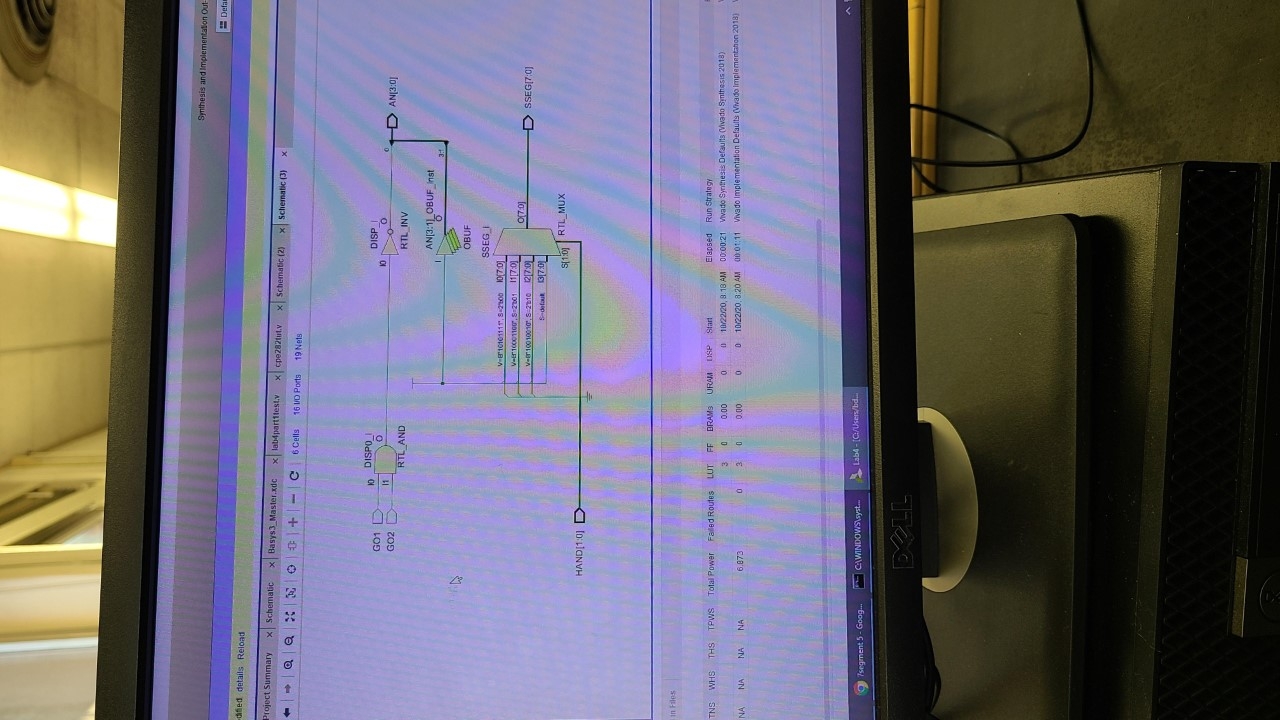
\includegraphics[width=15cm,height=15cm]{rtl}\newline
    (RTL)\end{center}
    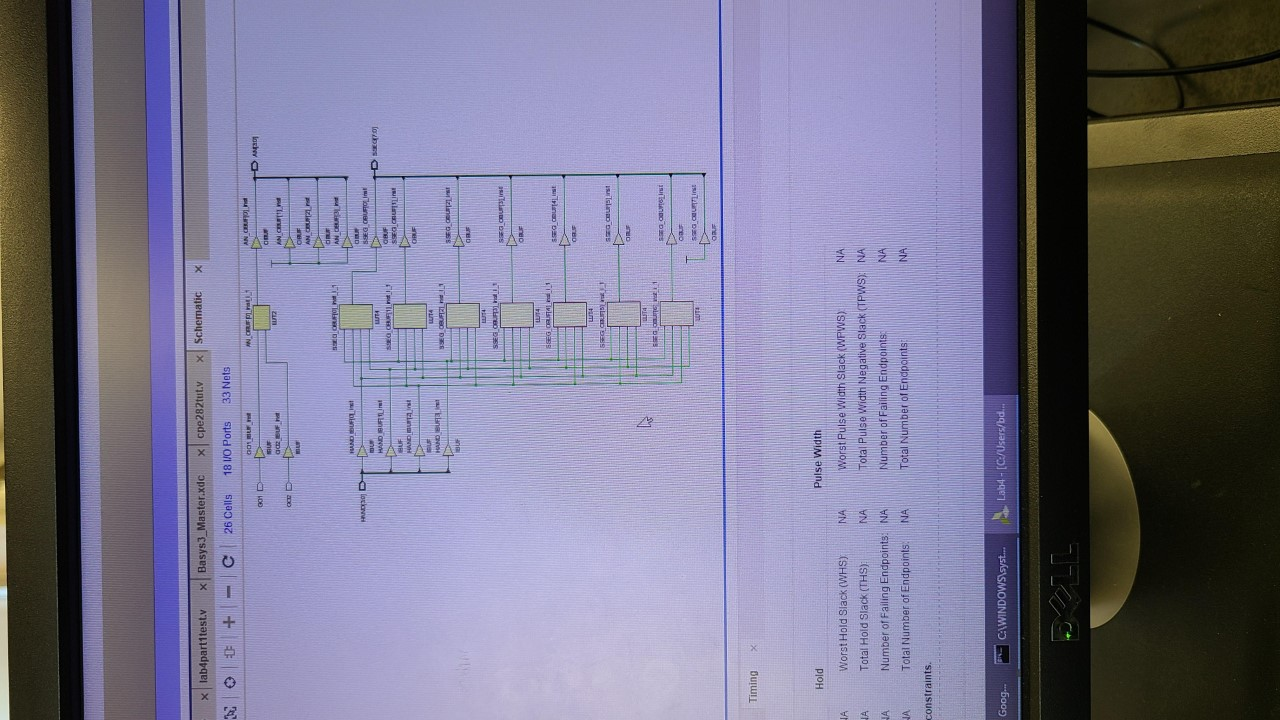
\includegraphics[width=15cm,height=15cm]{imp}\newline
(Implementation)
\end{document}

